\documentclass[crop,tikz,10pt]{standalone}
\usepackage{tikz}
	\usetikzlibrary{shapes}
	\usetikzlibrary{automata}
	\usetikzlibrary{arrows}
	\usetikzlibrary{backgrounds}
	\usetikzlibrary{calc}
	\usetikzlibrary{positioning}
	\usetikzlibrary{patterns}
	\usetikzlibrary{decorations.pathmorphing}
	\usetikzlibrary{decorations.pathreplacing}

\usepackage[scaled]{helvet}
\renewcommand{\familydefault}{\sfdefault}

\usepackage{booktabs}
\usepackage{bm}
\usepackage{siunitx}
\usepackage{xcolor}
    \definecolor{TUMOrange}{RGB}{227, 114, 34}
    \definecolor{TUMBlueDark}{RGB}{0, 82, 147}

\input{../../../../../resources/latex/_symbols.qmd}

\begin{document}

\newcommand{\n}[1]{\begin{tabular}{c}#1\end{tabular}}
\renewcommand{\vec}[1]{\boldsymbol{\mathbf{#1}}}
    
\pgfdeclarelayer{background}
\pgfdeclarelayer{foreground}

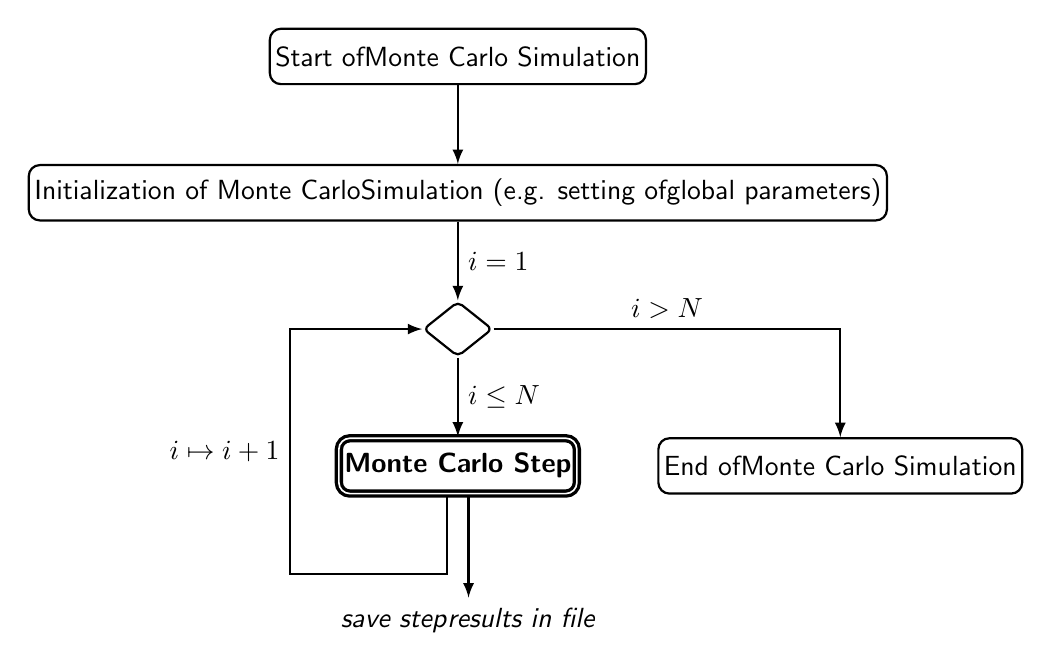
\begin{tikzpicture}[
    main/.style={draw, thick, rounded corners=4pt, inner sep=2pt, minimum size=20pt, minimum width=25pt, fill=white},
    decision/.style={draw, diamond, aspect=2, thick, rounded corners=2pt, inner sep=3pt, minimum size=20pt, minimum width=25pt, fill=white},
]

    %::. main nodes
    \node[main] (START) at (0,0) {\n{Start of\\Monte Carlo Simulation}};    
    \node[main, below = 1 of START] (INIT) {\n{Initialization of Monte Carlo \\ Simulation (e.g. setting of \\ global parameters)}};
    \node[decision, below = 1 of INIT] (CHECKSTEP) {};
    \node[main, below = 1 of CHECKSTEP, very thick, double] (STEP) {\n{\vspace{5mm}\\\textbf{Monte Carlo Step}\\\vspace{5mm}}};
    \node[main, right = 1 of STEP] (END) {\n{End of\\Monte Carlo Simulation}};


    %::. connections
    \draw[-latex, thick] (START) -- (INIT);
    \draw[-latex, thick] (INIT) -- node[midway, right] {$i=1$} (CHECKSTEP);
    \draw[-latex, thick] (CHECKSTEP) -- node [midway, right] {$i\leq N$} (STEP);
    \draw[-latex, thick] (STEP.250) |- ($(STEP.250) + (-2, -1)$) |- node[near start, left] {$i\mapsto i+1$} (CHECKSTEP.180);
    \draw[-latex, thick] (STEP.290) -- ($(STEP.290) + (0, -1.3)$) node[at end, below] {\n{\emph{save step }\\\emph{results in file}}};
    \draw[-latex, thick] (CHECKSTEP.0) -| node[near start, above] {$i>N$} (END.90);

\end{tikzpicture}

\end{document}